\chapter{Experiments}

\section{Classical Computer Vision-based Approach}

\subsection{Gaze Projection}
\begin{figure}
    \centering
    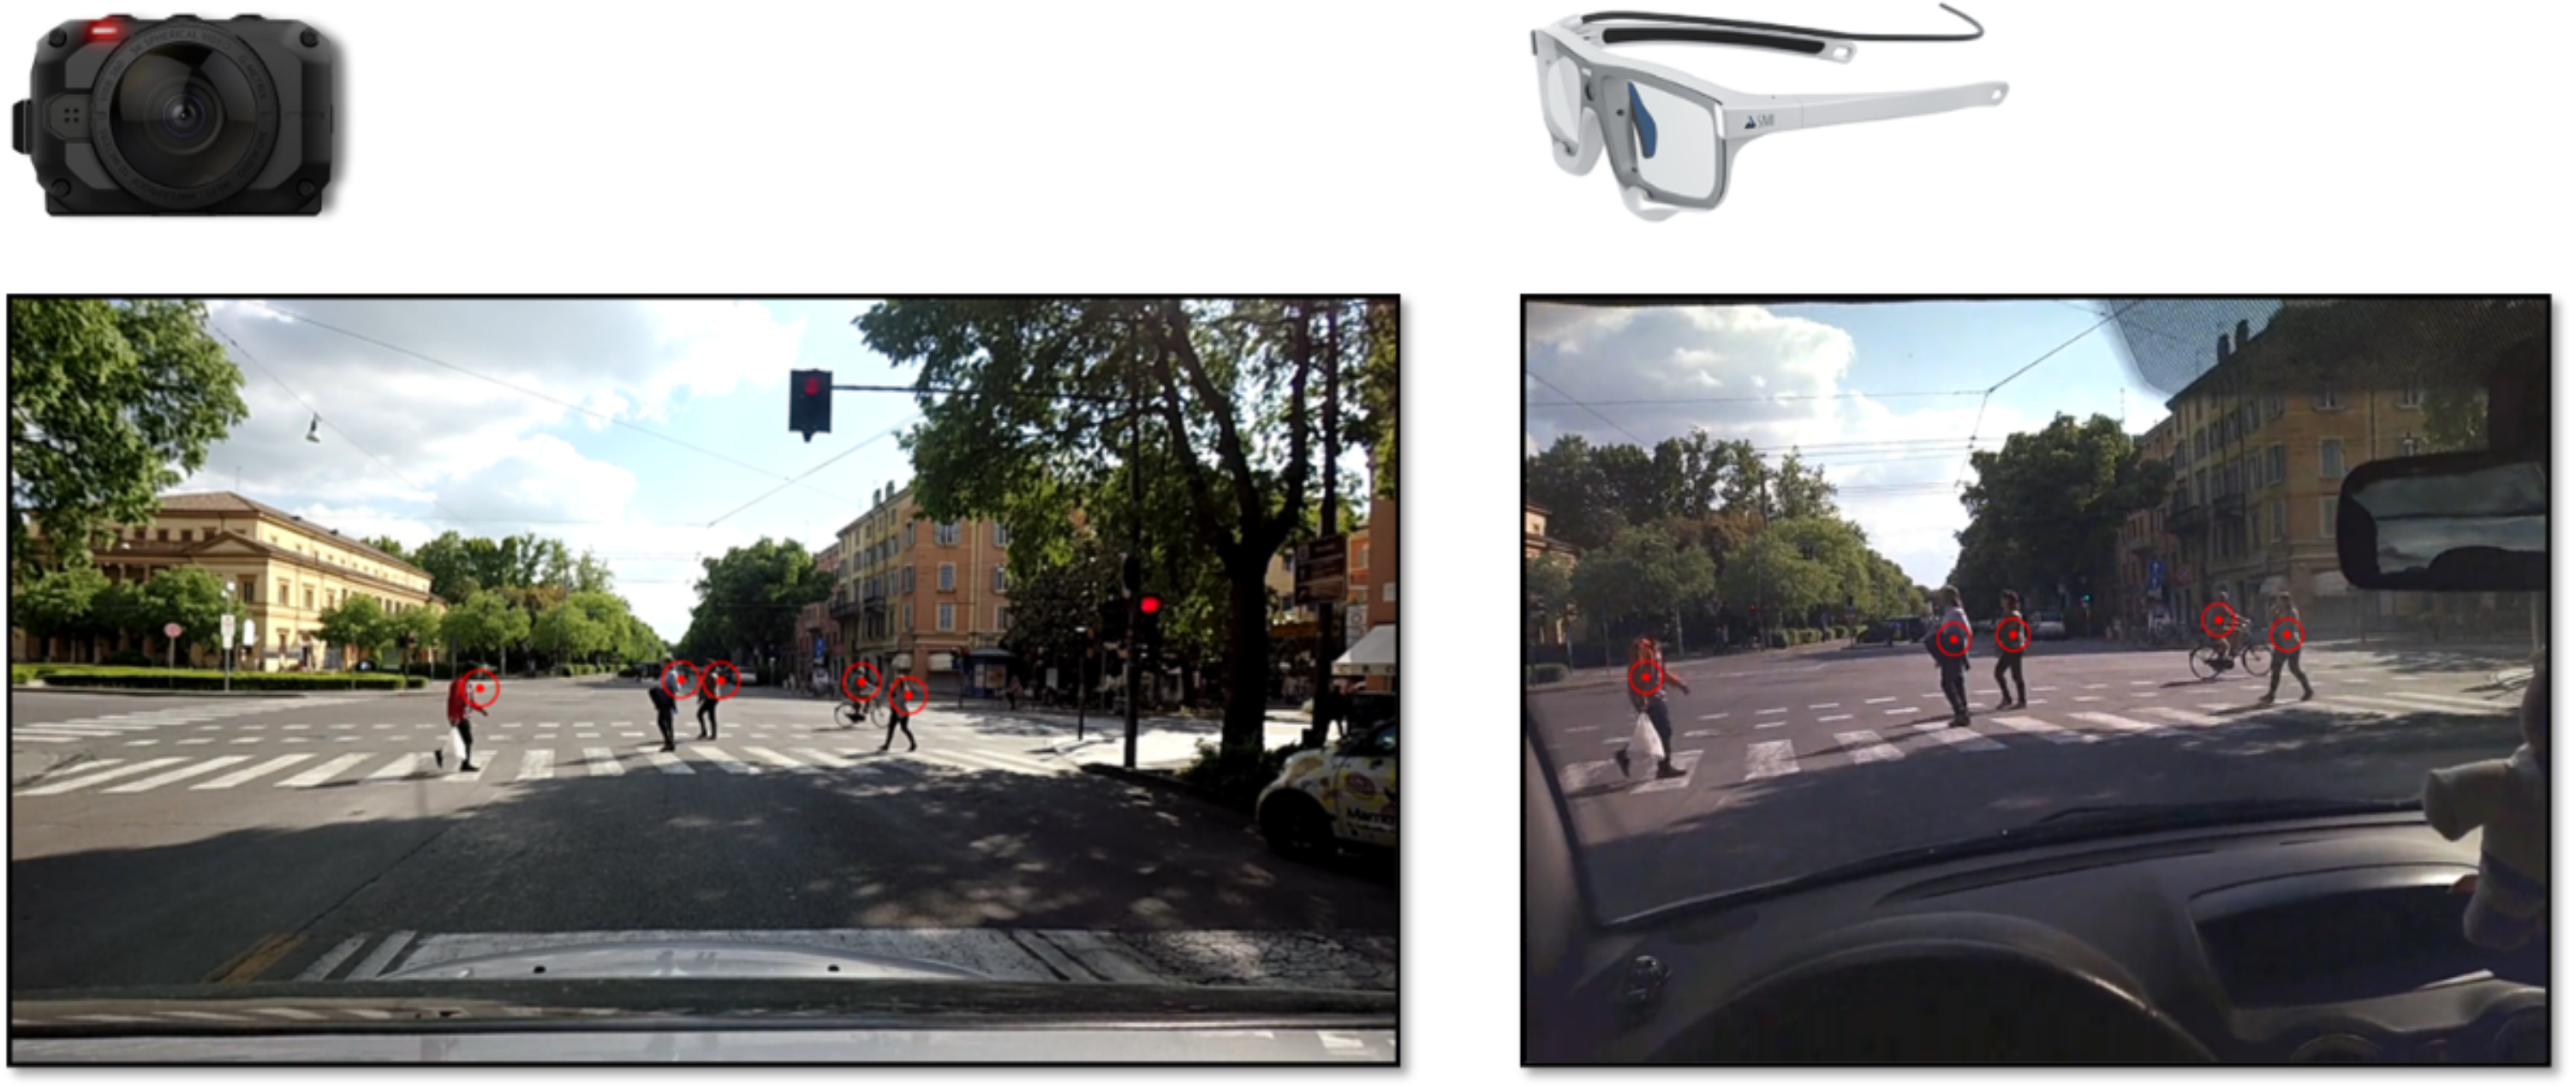
\includegraphics[width=\textwidth]{images/dreyeve/gaze_projection.png}
    \caption{Projection of the gaze from the ETG camera to the RT camera. 
    All the gaze points are manually set.
    \textbf{Left}: Roof top camera view.
    \textbf{Right}: ETG camera view.}
    \label{fig:gaze_projection}
\end{figure}
\begin{figure}
    \centering
    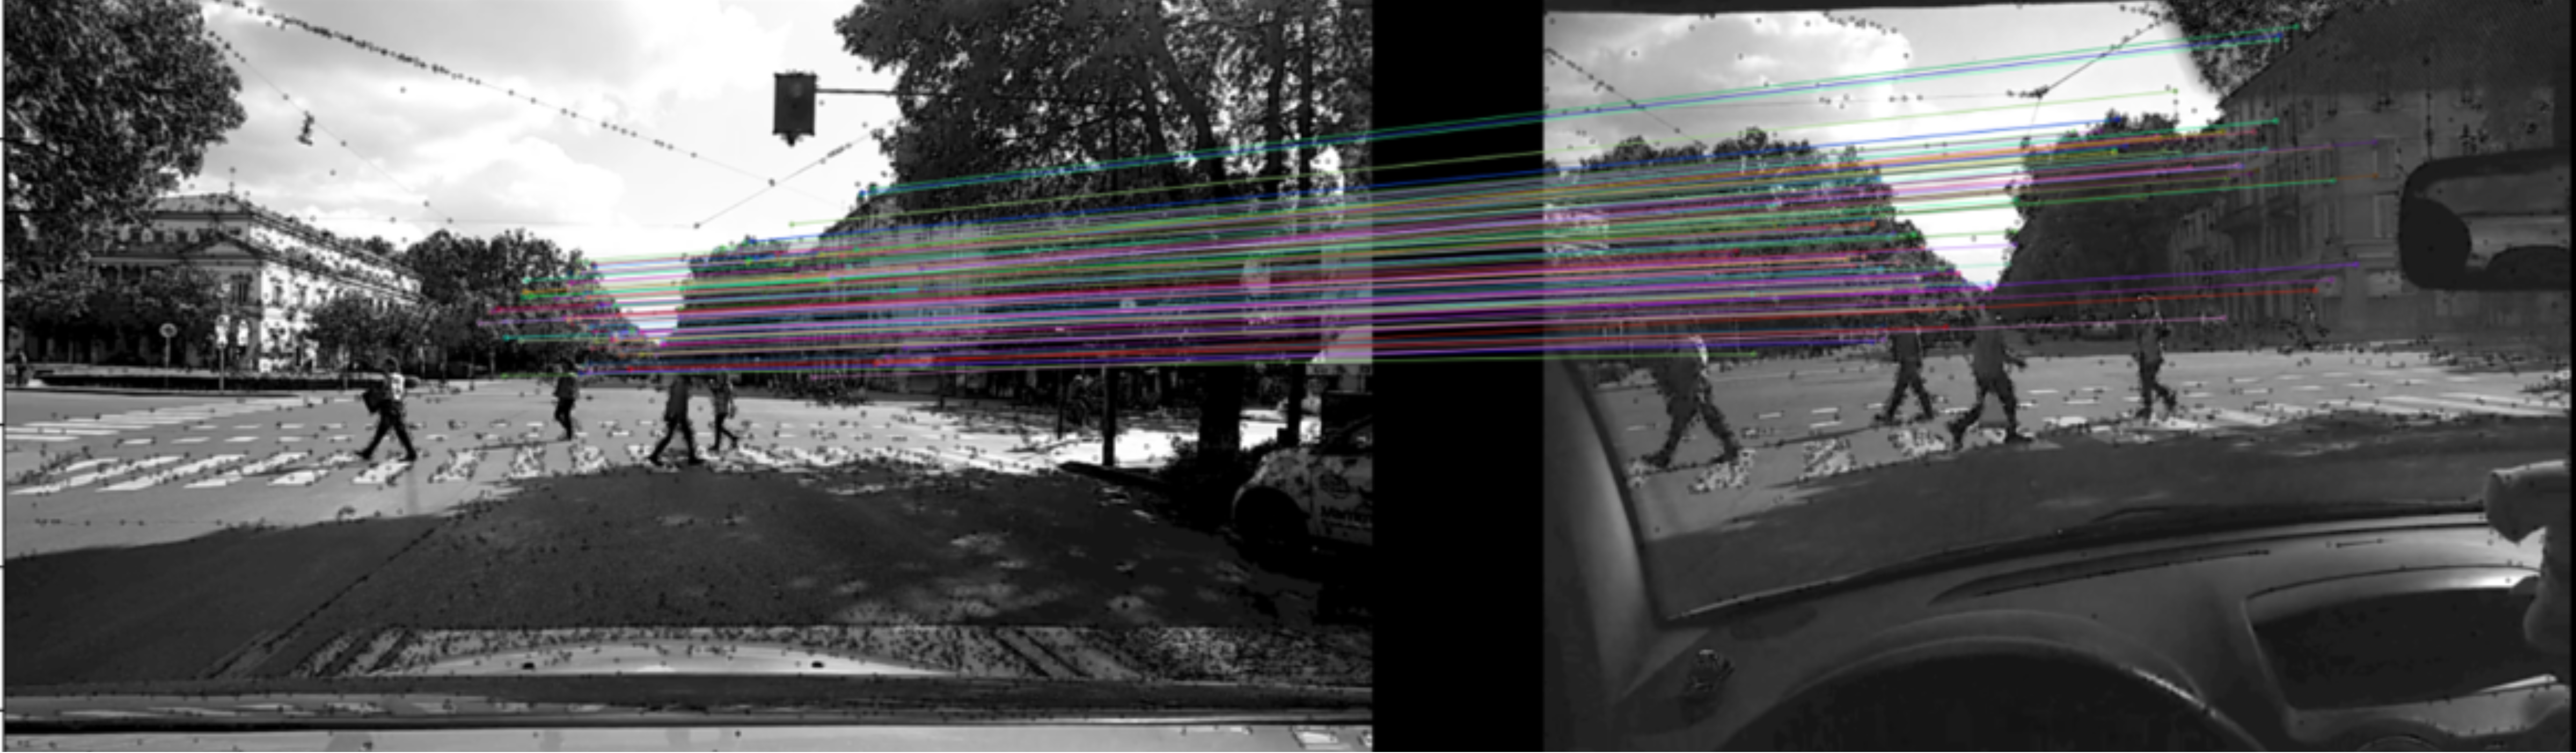
\includegraphics[width=\textwidth]{images/dreyeve/gaze_matchings.png}
    \caption{Projection of the gaze from the ETG camera to the RT camera. 
    All the gaze points are manually set.
    \textbf{Left}: Roof top camera view.
    \textbf{Right}: ETG camera view.}
    \label{fig:gaze_matchings}
\end{figure}
The projection of the gaze from the ETG camera to the RT camera is shown in 
Figure \ref{fig:gaze_projection}. We manually set some gaze points on the 
ETG camera such that they overlap with the vulnerable users. In this way, 
we are setting some operation points that we can use to evaluate the quality 
of the homography estimation. From the figure it is possible to see that the 
projection is not perfect, but it is a good approximation of the gaze in the 
RT camera plane. The small errors are due to the fact that the scene is not 
flat and the homography is a planar transformation. However, most pixels with 
high contrast correspond to objects that are far away from the vehicle, 
therefore the approximation is reasonable.

\subsection{Distribution of People in Dr(eye)ve}
\subsection{Gaze Interaction with Targets}
\subsection{Adding Depth Information}
\subsection{Adding Spatial Information}


\section {Deep Learning-based Approach}
\subsection {Data Distribution of BDD100k}
\subsection{Supervised Training on Dr(eye)ve}
\subsection{Semi-Supervised Training on Dr(eye)ve}
\subsection{Supervised Training on BDD100k}
\subsection{Semi-Supervised Training on BDD100k}

\subsection{Experiments with GPT4-o}
In May 2024 OpenAI released GPT4-o, their multilingual, multimodal generative 
pre-trained transformer. Considering its powerful capability to describe general 
contexts in wide scenes, we decided to test the architecture to solve a problem 
similar to ours. Experiments were conducted on BDD100k dataset.

\subsubsection{Problem Definition}
We defined two groups of six images each. The first group consists of general 
driving scenarios that contain at least one person in each image. 
The second group, on the other hand, is still related to driving scenarios but 
does not contain any person. However, in most images of both groups there are 
some common objects, including cars, buildings, etc.
Then the model will be asked to evaluate a new, never seen, image and answer 
in which group it belongs.

Other experiments in the two groups were done, including asking the model which 
common targets are present in each group.

\subsubsection{Data Selections}
\setlength{\subfigwidth}{45mm}
\setlength{\horspace}{.3\textwidth}
\begin{figure}
    \centering
    \begin{tabular}{p{\horspace} p{\horspace} p{\horspace}}
    \begin{subfigure}[b]{\subfigwidth}
        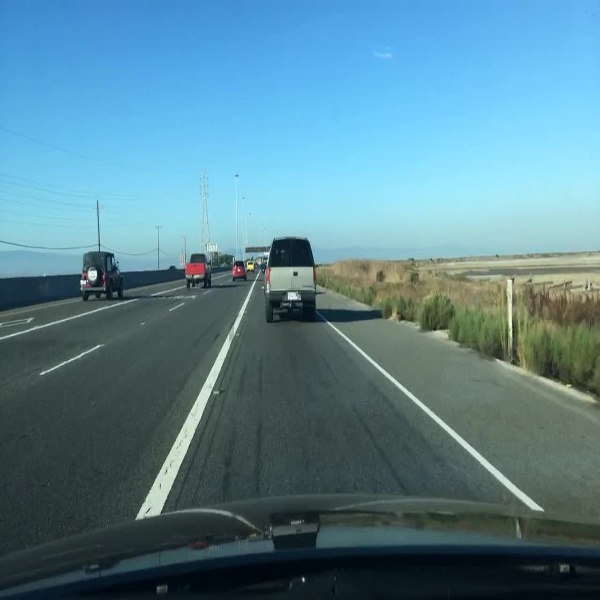
\includegraphics[width=\subfigwidth]{images/gpt4/s1.jpg}
    \end{subfigure}
    \hfill &
    \begin{subfigure}[b]{\subfigwidth}
        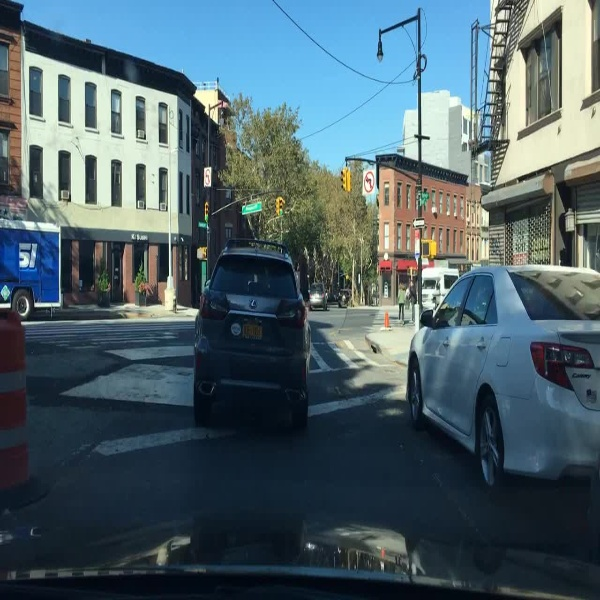
\includegraphics[width=\subfigwidth]{images/gpt4/s2.jpg}
    \end{subfigure} 
    \hfill &
    \begin{subfigure}[b]{\subfigwidth}
        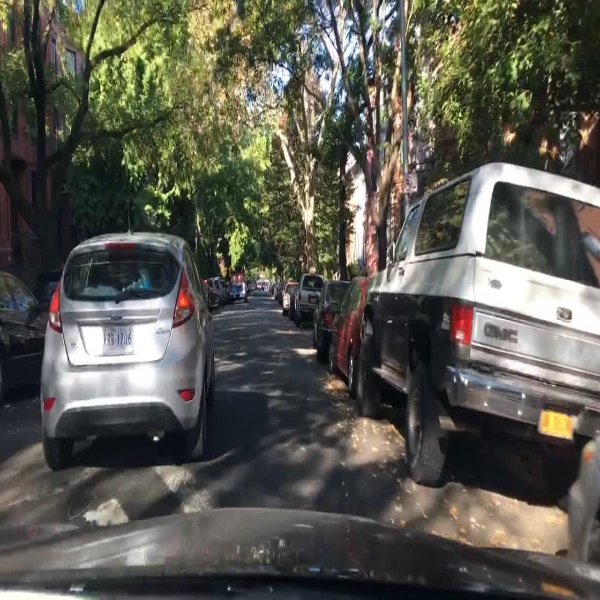
\includegraphics[width=\subfigwidth]{images/gpt4/s3.jpg}
    \end{subfigure} \\
    %
    \begin{subfigure}[b]{\subfigwidth}
        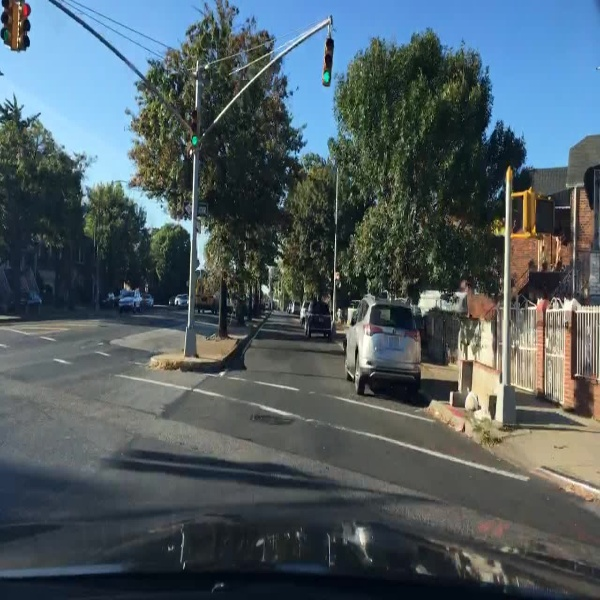
\includegraphics[width=\subfigwidth]{images/gpt4/s4.jpg}
    \end{subfigure}
    \hfill &
    \begin{subfigure}[b]{\subfigwidth}
        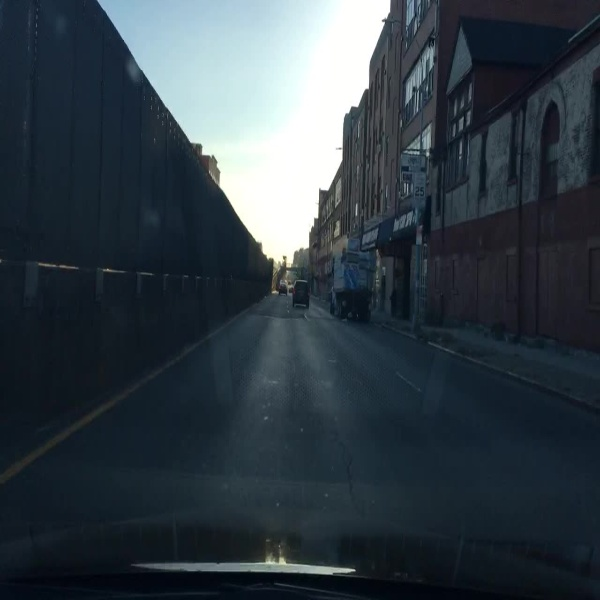
\includegraphics[width=\subfigwidth]{images/gpt4/s5.jpg}
    \end{subfigure} 
    \hfill &
    \begin{subfigure}[b]{\subfigwidth}
        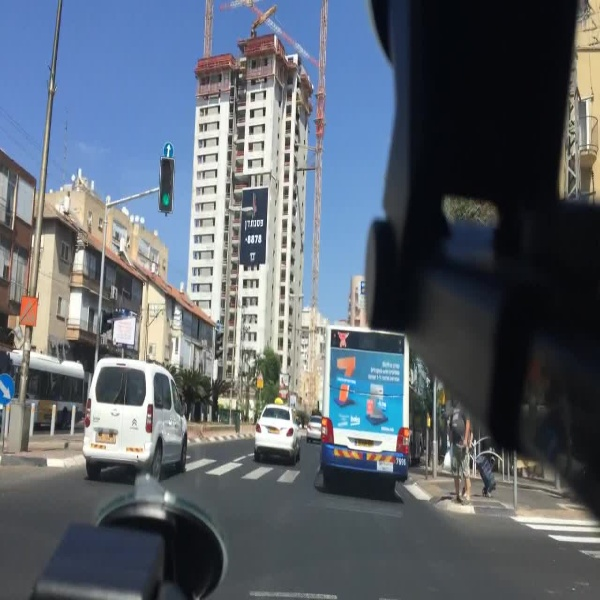
\includegraphics[width=\subfigwidth]{images/gpt4/s6.jpg}
    \end{subfigure}
\end{tabular}
\caption{Group of safe images, there are no people in all the images.}
\label{fig:safe_group}
\end{figure}
%
\begin{figure}
    \centering
    \begin{tabular}{p{\horspace} p{\horspace} p{\horspace}}
    \begin{subfigure}[b]{\subfigwidth}
        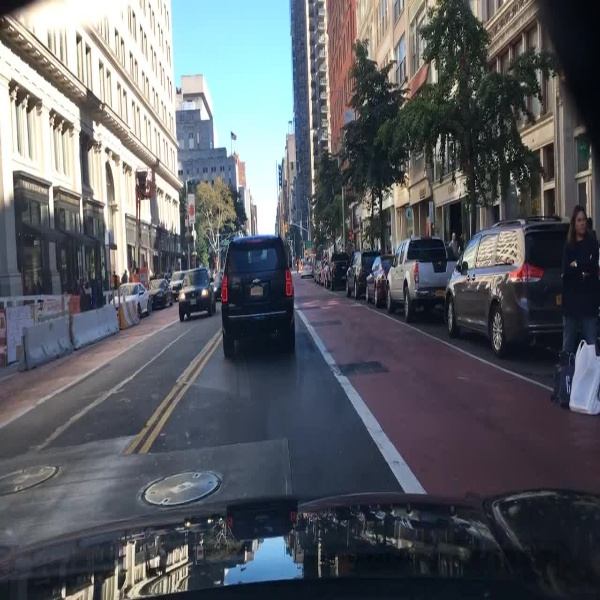
\includegraphics[width=\subfigwidth]{images/gpt4/d1.jpg}
    \end{subfigure}
    \hfill &
    \begin{subfigure}[b]{\subfigwidth}
        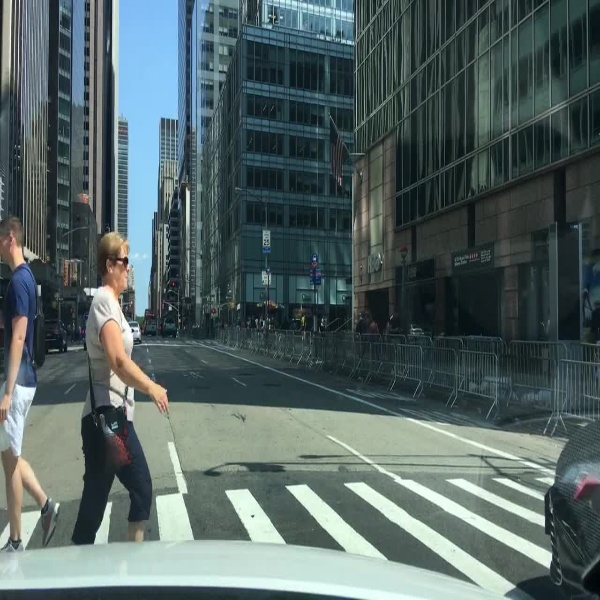
\includegraphics[width=\subfigwidth]{images/gpt4/d2.jpg}
    \end{subfigure} 
    \hfill &
    \begin{subfigure}[b]{\subfigwidth}
        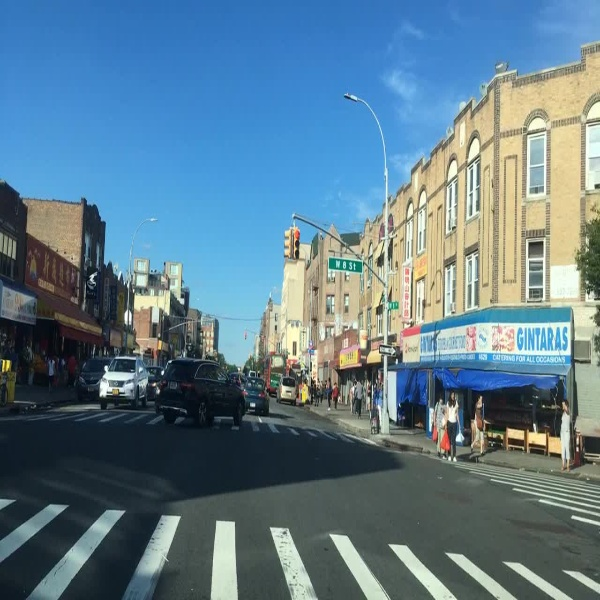
\includegraphics[width=\subfigwidth]{images/gpt4/d3.jpg}
    \end{subfigure} \\
    %
    \begin{subfigure}[b]{\subfigwidth}
        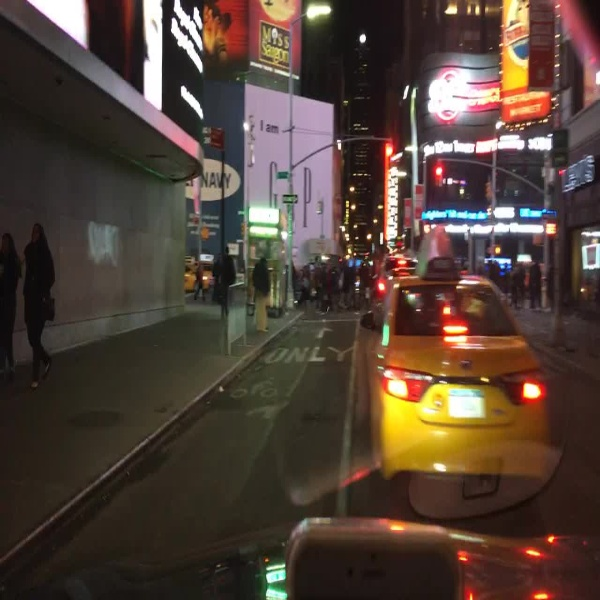
\includegraphics[width=\subfigwidth]{images/gpt4/d4.jpg}
    \end{subfigure}
    \hfill &
    \begin{subfigure}[b]{\subfigwidth}
        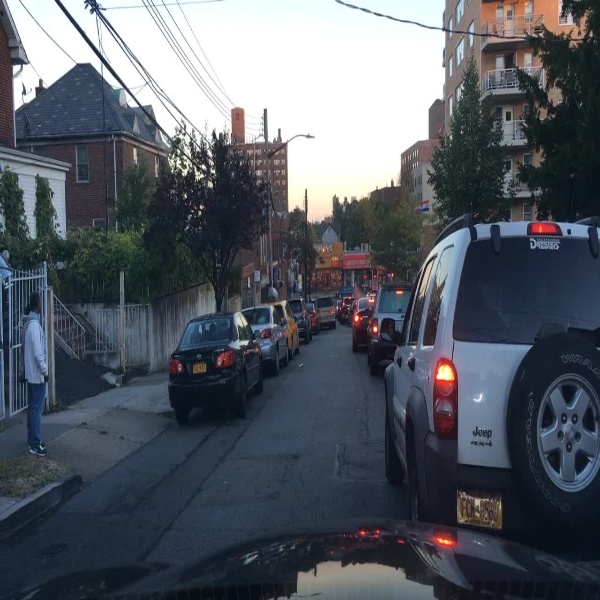
\includegraphics[width=\subfigwidth]{images/gpt4/d5.jpg}
    \end{subfigure} 
    \hfill &
    \begin{subfigure}[b]{\subfigwidth}
        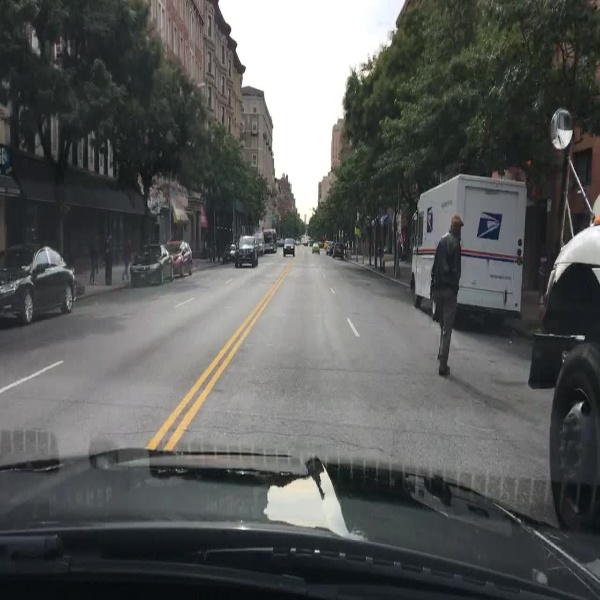
\includegraphics[width=\subfigwidth]{images/gpt4/d6.jpg}
    \end{subfigure}
\end{tabular}
\caption{Group of dangerous images, there are some people in each image.}
\label{fig:dangerous_group}
\end{figure}
The first group of images is shown in Figure \ref{fig:safe_group}. It consists 
of six images that do not contain any person. In particular, in the first image 
on the top left there is the ego-vehicle in a highway with some other vehicles 
on the front. The second on the top-center represents a downtown scenario with 
some vehicles on the front. In the third image on top-right there is a vehicle 
on the front and many vehicles parked on both sides of the road. The fourth 
image on bottom-left represents the ego-vehicle driving on a road with a traffic 
divider and some cars parked on the right side. In the fifth image on the 
bottom-center there is a straight road with some vehicles on the front and tall 
buildings on the sides. The last image on the bottom-right represents a 
downtown scenario with some vehicles, including cars and a bus. There is 
actually an occluded person in the image, but it is almost not visible.

The second group of images is shown in Figure \ref{fig:dangerous_group}. 
In the first image on the top-left there are two cars in fron of the ego-vehicle, 
some cars parked on both sides and a pedestrian standing on the right side. There 
are also some other pedestrians far away on sidewalks, not much visible in the 
image.
The second image on the top-center represents a downtown scenario where some 
pedestrians are crossing the road. There is also a car partially visible on the 
right of the ego-vehicle. The environment is characterized by tall buildings.
The third image on the top-right represents a downtown scenario with some 
empty crosswalks but many pedestrians on sidewalks. There are also some cars 
driving on the main road.
The fourth image on the bottom-left represents a night downtown scenario with a 
taxi in front of the ego-vehicle and group of pedestrians on the left sidewalk 
and far away, where there are crosswalks and red traffic lights.
In the fifth image, bottom-center, there is a line of cars in front of the 
ego-vehicle, some cars parked on the left side, and a pedestrian standing on the 
left sidewalk.
The last image on the bottom-right represents a main road with some vehicles 
parked on both sides, some others driving, and a person standing on the right 
side of the road.

Considering the dangerous scenarios, some specific cases were carefully selected,
especially with people partially visible, in the corners of the images, and 
on the background. On the other hand, in both groups there are many vehicles, both 
in foreground and background, that contribute to add noise to the data to 
classify.
This decision represents a further challenge for the model to 
isolate the right group of pixels.